%The Enriched Xenon Observatory \cite{Hall:2010zzg} will search for \bbonu\ in \XE. The ultimate goal of the Collaboration is the development of the barium tagging for a multi-ton xenon-based detector, which would lead to a virtually background-free experiment. Prior to that, the Collaboration has built the EXO-200 detector, a $\sim$200-kg liquid xenon (enriched to 80.6\% in \XE) time projection chamber that detects both scintillation and ionization.
%
%The fiducial volume of the chamber, 44 cm in length, is divided in two halves by a central cathode (see fig.~\ref{fig:exo}, left). Ionization charges created in the xenon by charged particles drift under the influence of an electric field towards the two ends of the chamber. There, the charge is collected by a pair of crossed wire planes which measure its amplitude and transverse coordinates. Each end of the chamber includes also an array of avalanche photodiodes (APDs) to detect the 178-nm scintillation light produced by primary interactions. The sides of the chamber are covered with teflon sheets that act as VUV reflectors, improving the light collection. The simultaneous measurement of both the ionization charge and scintillation light of the event may in principle allow to reach a detector energy resolution as low as 3.3\% FWHM at the \XE\ Q-value, for a sufficiently intense drift electric field \cite{EXO-200:2003bso}. 
%
%The xenon is held inside a thin copper vessel immersed in a cryofluid that also shields the experiment from external radioactive backgrounds. The HFE heat-transfer fluid is stored in a vacuum-insulated low-activity copper cryostat. The cryostat is surrounded on all sides by 25 cm of low-activity lead. The entire assembly is surrounded by a radon-free tent and housed in a class 100 clean room, the exterior of which is instrumented on five sides with plastic scintillator panels for vetoing cosmic rays with 95.9\% efficiency. The detector is located 2150 feet underground for an overburden of 1585 meters water equivalent, at WIPP (Waste Isolation Pilot Plant), in the United States.
%
%%%%%%
%\begin{figure}[t!]
%\begin{center}
%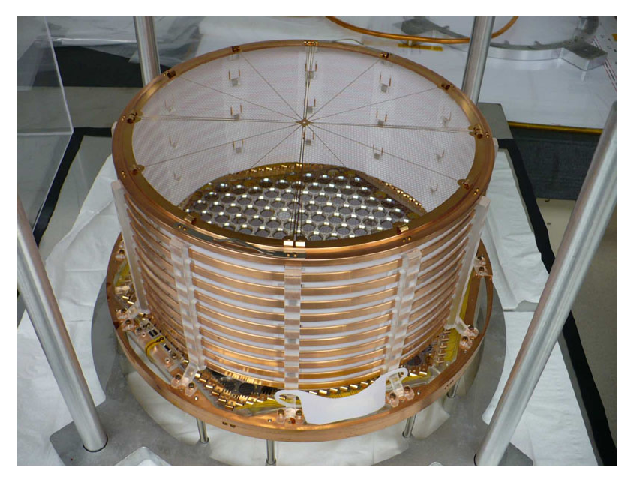
\includegraphics[width=0.475\textwidth]{img/exo1.eps}
%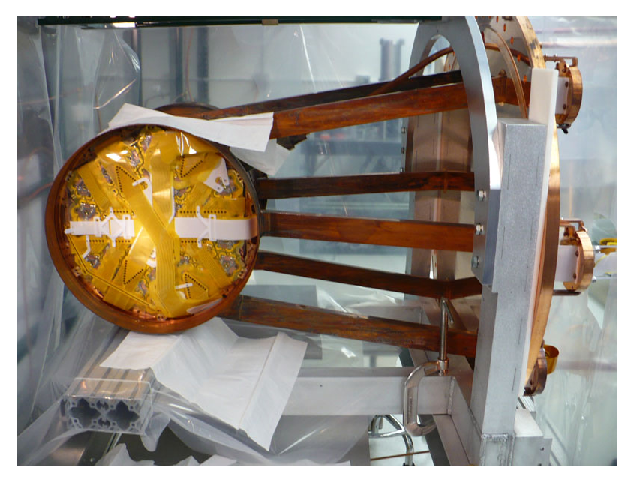
\includegraphics[width=0.475\textwidth]{img/exo2.eps}
%\end{center}
%\caption{Left: one half of the EXO chamber, viewed from the cathode plane. Right: the chamber attached to the cryostat door, as viewed from the bottom of the APD plane. The legs contain the readout cabling and are also the conduits for xenon circulation.} \label{fig:exo}
%\end{figure}
%%%%%%
%
%The EXO-200 TPC was installed in its cryostat in early 2010. The detector was first filled with natural (unenriched) xenon in late 2010. The data collected during these engineering runs were used to make a first assessment of the performance of the detector, and to perform a first round of calibrations. Low-background running with enriched xenon started in the spring of 2011. The EXO Collaboration announced the observation of the \bbtnu\ mode of \XE\ in August 2011. Prior to this measurement, reported in table~\ref{tab:bb2nu_exp}, the \bbtnu\ had been observed in all other important \bbonu\ candidate nuclei except \XE . The measured \bbtnu\ half-life is significantly lower than previously reported lower limits \cite{Bernabei:2002bn,Gavriljuk:2005xc}.
%
%To identify the daughter barium, several methods are under study, including single-ion fluorescence, resonant ionization spectroscopy (RIS), and mass spectroscopy. Single ion fluorescence is a highly sensitive and highly selective method to observe a barium ion while held under vacuum in a RF trap. In this technique, the Ba$^+$ ion is rapidly cycled from its $6^2\text{S}_{1/2}$ ground state to its $6^2\text{P}_{1/2}$ excited state by illuminating it with lasers of the appropriate wavelength (493 nm and 650 nm), see fig.~\ref{fig:bariumenergylevels}. As the electronic state changes, the laser photons are scattered in all directions, and the scattered light can be easily detected by a photo-multiplier tube. EXO has achieved good single barium ion identification with this technique, even in the presence of low pressure xenon and helium gas mixtures. However, this technique also requires that the barium ion be retrieved from the TPC volume, transported to the RF trap, released, and trapped, while not altering its chemical or ionization state. Resonant ionization spectroscopy, on the other hand, is a technique which allows single barium ions to be observed without requiring a vacuum ion trap. In RIS, barium ions are desorbed from the surface of a transport probe, and subsequently resonantly ionized under illumination by 554 nm and 390 nm lasers. The ionized barium can then be observed with a Channeltron electron multiplier. Initial tests with the RIS technique have successfully identified barium being desorbed from the probe tip, so this technique is promising. Other avenues of research include barium identification within xenon ice, and barium extraction from a high pressure gas TPC using gas nozzles. 
% 


The nEXO neutrinoless double beta decay experiment is designed to use a time projection chamber and 5000 kg of isotopically enriched liquid xenon to search for the decay in 136Xe. This detector will be based on very successful EXO-200 detector. A single-phase liquid xenon TPC instrumented to read both scintillation and charge. The anti-correlation of these two signals allowed for an energy resolution of 2.89\% FWHM@Qbb \cite{EXO-200:2020wmu}.

This design also provided the capability of a good fidutialization of the events in the detector and, more important, certain capability to separate them by topology. In particular, the separation of single-site and multi-site events [cite] provided a strong background suppression.

The nEXO design aims to build a volume of 5 tonnes of enriched Xe136. The TPC vessel is a right copper cylinder with both inner height and diameter equal to 127.7 cm surrounded by 33,000 kg of HFE-7000, which serves as both thermal bath and radiation shield. A vacuum layer between an inner vessel and an outer vessel of the cryostat provides thermal insulation from an active water shield, referred to as the outer detector. The TPC itself will have 113.3 cm diameter by 118.3 cm drift height, creating a total xenon mass in the drift region of 3648 kg for an active mass of 3281 kg. This design requires 10 ms of electron life-time to guarantee good energy resolution when reading the ionisation signal. This is achieve by a good purification system and a relatively moderate drift field of 400 V/cm. \cite{nEXO:2021ujk}.



%%%%%%
\begin{figure}[t!]
\begin{center}
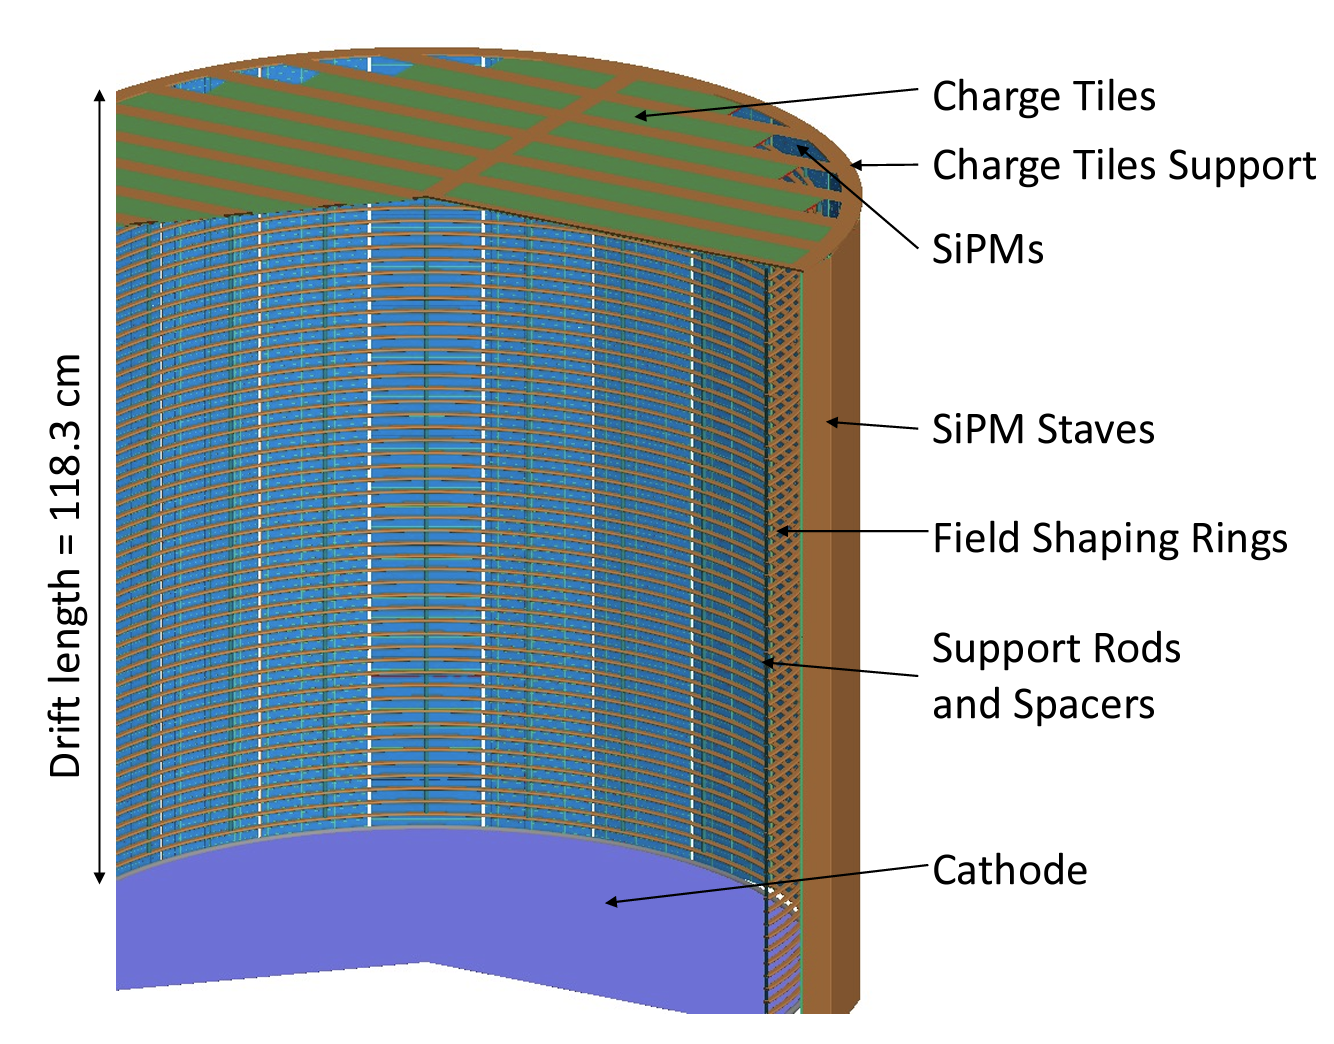
\includegraphics[width=0.475\textwidth]{img/nexo_design}
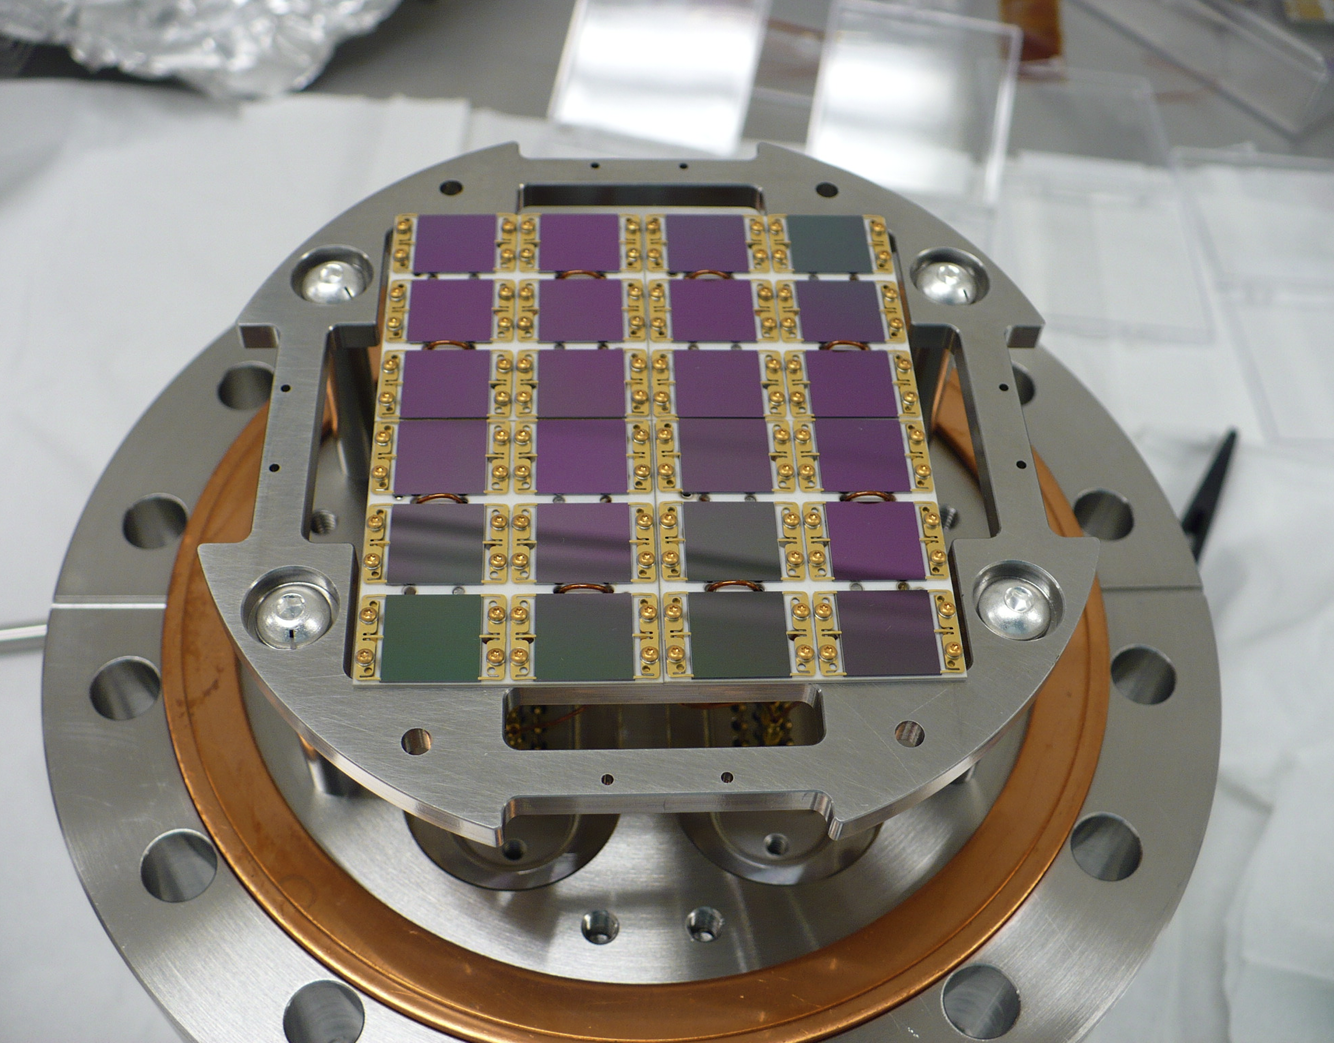
\includegraphics[width=0.475\textwidth]{img/nexo_sipms}
\end{center}
\caption{Left: Close up view of the main components inside the nEXO TPC vessel. Right: Test array of 24 SiPMs used to be used together with charge collection tiles in LXe.Each SiPM is cm$^2$.} \label{fig:nexo}
\end{figure}

Efficient scintillation light collection is an essential requisite for nEXO to attain proper energy resolution and to provide the start time to localize events along the drift field. Actually, in order to reach <2.35\% FWHM energy resolution, the overall optical efficiency must be 3\%  or higher, this is achieved by using SiPMs arrays operated directly in the liquid xenon behind the TPC field shaping rings. The SiPM will have ~1cm$^2$ active area and will be mounted in 24 long staves surrounding the TPC field cage. The necessity of reading as much light as possible has a relevant impact on the TPC design. In particular, the field cage must be as transparent as possible allowing the photons to reach the photsensors region. This affect the geometry of the rings, as they need to be thiner. Also, a coating of vacuum deposited aluminum, protected against oxidation by a layer of MgF2 will make all rings reflective to VUV. In addition, it will allow to remove the traditional PTFE reflective panels used in other liquid xenon TPCs, thus reducing the amount of materials and outgassing inside the detector volume.

One of the main tools the nEXO collaboration proposes to reduce the level of background events is the based on taking advantage of the relatively short attenuation length of $\gamma$-ray at 2.4 MeV energy in LXe, of only 8.7 cm. By selecting a region in the most inner part of the detector they can further reduce the background rate by almost an order of magnitude in the most inner ton of active material. Adding this technique to the energy resolution and topological separation nEXO is predicted to achieve a background rate of 3.6 × 10$^{-4}$ cts/(FWHM·kg·y) in the inner 2000 kg of LXe. 

With this level of background nEXO aims to reach a sensitivity of 9.2 × 10$^{27}$ yrs at 90\% C.L. after 10 years of operation and, an expected 3 sigma discovery potential of 5.7 × 
10$^{27}$ yrs \cite{nexocprecdr}. However, in a recent document \cite{nEXO:2021ujk} the nEXO Collaboration claims for an improved design and understanding of the nEXO design, together with the development of a \bbonu\ DNN discriminator that pushes the background index to 
b=7×10$^{-5}$ cts/(FWHM·kg·yr) obtaining a half-life sensitivity of 1.35×10$^{28}$ 
yr at 90\% C.L.